\documentclass{article}\usepackage{hyperref}\usepackage{graphicx}\usepackage{amsmath}\usepackage{amsfonts}\newcommand{\deq}{\stackrel {\rm def}{=}}\newcommand{\gtlt}{\stackrel {>}{<}} \newcommand{\ltgt}{\stackrel {<}{>}} \newcommand{\eqline}[1]{\\\centerline{$#1$}\\}\newcommand{\tab}{\hphantom{6mm}}\newcommand{\well}[1]{\vspace{0.3cm}\hspace{-2cm}{\tt #1}} \begin{document}

\section*{Equivalence between softmax and prototypes classification}

Let us consider an affine softmax function:
\eqline{{}_\tau\nu_l\left({\bf x}\right) \deq \frac{\exp(f_l({\bf x})/\tau)}{\sum_{j'} \exp(f_{j'}({\bf x})/\tau)}} with $f_l({\bf x}) \deq {\bf w}_l^T \, {\bf x} + w^0_l$ and the decision rule
\eqline{l_{\bf x} = \mbox{arg max}_{l'} {}_\tau\nu_{l'}\left({\bf x}\right)}

This yields a piece-wise linear segmentation of the feature space, since:
\eqline{\small \begin{array}{lrcl}
&{}_\tau\nu_{l}\left({\bf x}\right) &\gtlt& {}_\tau\nu_{l'}\left({\bf x}\right) \\
\Leftrightarrow&
\frac{\exp(f_l({\bf x})/\tau)}{\sum_{l''} \exp(f_{l''}({\bf x})/\tau)} &\gtlt& 
\frac{\exp(f_{l'}({\bf x})/\tau)}{\sum_{l''} \exp(f_{l''}({\bf x})/\tau)} \\
\Leftrightarrow&
\exp(f_l({\bf x})/\tau) &\gtlt& \exp(f_{l'}({\bf x})/\tau)\\
\Leftrightarrow&
f_l({\bf x}) &\gtlt& f_{l'}({\bf x})\\
\end{array}}
the denominators being identical and the exponential being a strictly increasing function.
Writing ${\bf w}_{ll'} = {\bf w}_l - {\bf w}_{l'}$ we obtain:
\eqline{l_{\bf x} = \{l, \forall l' \ne l, {\bf w}_{ll'}^T \, {\bf x} +  w^0_{ll'} \geq 0\}}
for the $L\,(L-1)/2$ category pairs.

For each inequality we may consider any pair of point ${\bf p}_{ll'}, {\bf p}_{l'l}$ for which the separation hyperplane defined by ${\bf w}_{ll'}^T \, {\bf x} +  w^0_{ll'} = 0$ is the median, i.e., from a few elementary algebra:\\
\begin{tabular}{cc}
\parbox[u]{0.5\textwidth}{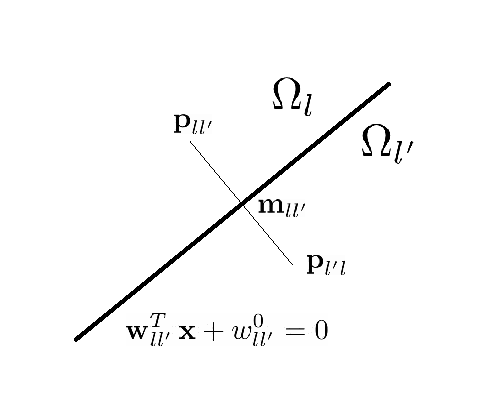
\includegraphics[width=0.5\textwidth]{img/softmax-median}}
&
$\begin{array}{rcl}
{\bf p}_{ll'} &\deq& {\bf m}_{ll'} + \lambda \, {\bf w}_{ll'} \\
{\bf p}_{l'l} &\deq& {\bf m}_{ll'} - \lambda \, {\bf w}_{ll'} \\
{\bf m}_{ll'} &\deq& {\bf w}_{ll'}^\perp - \alpha \, {\bf w}_{ll'}\\
\alpha &\deq& w^0_{ll'} / \|{\bf w}_{ll'}\|^2 \\
\end{array}$
\end{tabular}\\
for any $\lambda > 0$ and any vector ${\bf w}_{ll'}^\perp, {\bf w}_{ll'} \perp {\bf w}_{ll'}^\perp= 0$, yielding: 
\eqline{\small \begin{array}{lrcl}
&d({\bf x}, {\bf p}_{ll'})  &\ltgt& d({\bf x}, {\bf p}_{l'l}) \\
\Leftrightarrow&
d({\bf x}, {\bf p}_{ll'})^2  &\ltgt& d({\bf x}, {\bf p}_{l'l})^2 \\
\Leftrightarrow&
\|{\bf x}\|^2 - 2 {\bf p}_{ll'}^T \, {\bf x} + \|{\bf p}_{ll'}\|^2 
 &\ltgt&
\|{\bf x}\|^2 - 2 {\bf p}_{l'l}^T \, {\bf x} + \|{\bf p}_{l'l}\|^2 \\
\Leftrightarrow&
-2 ({\bf p}_{ll'} - {\bf p}_{l'l})^T \, {\bf x} + \|{\bf p}_{ll'}\|^2 - \|{\bf p}_{l'l}\|^2 &\ltgt& 0 \\
\Leftrightarrow&
-4 \, \lambda \, {\bf w}_{ll'}^T \, {\bf x} + \|{\bf p}_{ll'}\|^2 - \|{\bf p}_{l'l}\|^2 &\ltgt& 0 \\
\Leftrightarrow&
-4 \, \lambda \, {\bf w}_{ll'}^T \, {\bf x} - 4 \, \alpha \, \lambda \|{\bf w}_{ll'}\|^2 &\ltgt& 0 \\
\Leftrightarrow&
-4 \, \lambda \, \left( {\bf w}_{ll'}^T \, {\bf x} +  w^0_{ll'} \right) &\ltgt& 0 \\
\Leftrightarrow&
{\bf w}_{ll'}^T \, {\bf x} +  w^0_{ll'}  &\gtlt& 0 \\
\end{array}}
These pairs of point ${\bf p}_{ll'}, {\bf p}_{l'l}$ are thus defined up to $N \, L\,(L-1)/2$ degrees of freedom ($\lambda$ and ${\bf w}_{ll'}^\perp \in {\cal R}^N$ subject to an orthogonality constraint, for each category pair).

A step further, from a geometrical point of view, it is coherent to require that $l_{{\bf p}_{ll'}} = l$, in words that each prototype belongs to a polytope $\Omega_l$ corresponding to the label $l$, i.e., that $\forall l,l',l'' l \ne l', l \ne l'', {\bf w}_{ll''}^T \, {\bf p}_{ll'} +  w^0_{ll''} > 0$. This corresponds to a linear programming problem with $N\,L$ degrees of freedom and $(L\,(L-1)/2)^2$ inequalities, thus with solutions in the general case as soon as $N > L^3/4 + O(L^2)$, i.e., as soon as the number of features is high enough with respect to the number of categories.

Is this possible to reduce the number of prototypes, i.e., that ${\bf p}_{ll'} \stackrel {?}{=} {\bf p}_{ll''}$ for some of the $L\,(L-1)$ prototypes ? This generates $N$ additional linear constraints for each merge, and the non trivial fact that prototype pairs are to live into the same connex component of a given $\Omega_l$ has to be taken into account. A simple count of the number of degree of freedom shows that the number of constraints is in the general case twice the number of possible adjustmnt. Prototype merge is thus possinle, but not completely.

The softmax decision rules is thus equivalent to a nearest-neighbor algorithm considering $O(L^2)$ prototypes.

\bibliographystyle{alpha}\bibliography{../bib/vthierry} \end{document}
